% coding:utf-8

%----------------------------------------
%FOSAPHY, a LaTeX-Code for a summary of basic physics
%Copyright (C) 2013, Daniel Winz, Ervin Mazlagic

%This program is free software; you can redistribute it and/or
%modify it under the terms of the GNU General Public License
%as published by the Free Software Foundation; either version 2
%of the License, or (at your option) any later version.

%This program is distributed in the hope that it will be useful,
%but WITHOUT ANY WARRANTY; without even the implied warranty of
%MERCHANTABILITY or FITNESS FOR A PARTICULAR PURPOSE.  See the
%GNU General Public License for more details.
%----------------------------------------

\documentclass[a5paper,10pt,fleqn]{book}

\usepackage{fosaphy_layout}

\title{Formelsammlung Physik
% \\\textcolor{red}{\textbf{\Huge{Achtung! \\Diese Formelsammlung wird bis zur 
% Modul\-end\-prüfung nicht mehr erweitert. Wir empfehlen für die 
% Modulendprüfung das Taschenbuch Physik von Horst Kuchling oder die 
% Formelsammlung von Aurel Hunkeler. }}}
}

\author{Daniel Winz\\Ervin Mazlagi\'c\\Mario Felder\\Marcel Holzmann}
\date{\today~\dtc}

\begin{document}

\maketitle

% coding:utf-8

%----------------------------------------
%FOSAPHY, a LaTeX-Code for a summary of basic physics
%Copyright (C) 2013, Daniel Winz, Ervin Mazlagic

%This program is free software; you can redistribute it and/or
%modify it under the terms of the GNU General Public License
%as published by the Free Software Foundation; either version 2
%of the License, or (at your option) any later version.

%This program is distributed in the hope that it will be useful,
%but WITHOUT ANY WARRANTY; without even the implied warranty of
%MERCHANTABILITY or FITNESS FOR A PARTICULAR PURPOSE.  See the
%GNU General Public License for more details.
%----------------------------------------

\chapter*{Über diese Arbeit}
Dies ist das Ergebnis einer Zusammenarbeit auf Basis freier Texte erstellt von 
Studierenden der Fachhochschule Luzern und ist unter der GPLv2 lizenziert. Der 
\TeX - bzw. \LaTeX -Code ist auf \url{github.com/fosa/fosaphy} hinterlegt.Eine 
aktuelle PDF-Ausgabe steht auf \url{fosa.adinox.ch} zum Download bereit.

In dieser Formelsammlung sind die Inhalte des Physikteils der Module MA+PHY1T 
und MA+PHY2T der HSLU-T\&A zusammengefasst. 

Allfällige Fehler können per E-Mail an die Autoren 
(\href{mailto:info.fosa@gmail.com}{\nolinkurl{info.fosa@gmail.com}}) 
gemeldet werden. 


\tableofcontents

% coding:utf-8

%----------------------------------------
%FOSAPHY, a LaTeX-Code for a summary of basic physics
%Copyright (C) 2013, Daniel Winz, Ervin Mazlagic

%This program is free software; you can redistribute it and/or
%modify it under the terms of the GNU General Public License
%as published by the Free Software Foundation; either version 2
%of the License, or (at your option) any later version.

%This program is distributed in the hope that it will be useful,
%but WITHOUT ANY WARRANTY; without even the implied warranty of
%MERCHANTABILITY or FITNESS FOR A PARTICULAR PURPOSE.  See the
%GNU General Public License for more details.
%----------------------------------------

% coding:utf-8

%----------------------------------------
%FOSAPHY, a LaTeX-Code for a summary of basic physics
%Copyright (C) 2013, Daniel Winz, Ervin Mazlagic

%This program is free software; you can redistribute it and/or
%modify it under the terms of the GNU General Public License
%as published by the Free Software Foundation; either version 2
%of the License, or (at your option) any later version.

%This program is distributed in the hope that it will be useful,
%but WITHOUT ANY WARRANTY; without even the implied warranty of
%MERCHANTABILITY or FITNESS FOR A PARTICULAR PURPOSE.  See the
%GNU General Public License for more details.
%----------------------------------------

\chapter{SI Einheiten}

Das Internationale Einheitensystem, SI genannt 
(franz. \textit{Système international d'inités}),
ist ein kohärentes dezimales und metrisches Einheitssystem für 
physikalische Grössen. Dieses wurde seit Ende des 18. Jahrhunderts
entwickelt und ist mittlerweile von jedem Staat offiziell eigeführt mit 
Ausnahme der USA, Myanmar und Liberia.

\newpage
\section{Grundeinheiten}
\begin{footnotesize}
\begin{tabular}{llll}
  \rowcolor{white} \textbf{Basisgrösse} & \textbf{Symbol} 
                    & \textbf{Einheit} & \textbf{Zeichen}\\
  \rowcolor{lgray} Länge       & $l$   & Meter     & $m$\\
  \rowcolor{white} Zeit        & $t$   & Sekunde   & $s$\\
  \rowcolor{lgray} Masse       & $m$   & Kilogramm & $kg$\\
  \rowcolor{white} Temperatur  & $T$   & Kelvin    & $K$\\
  \rowcolor{lgray} Stromstärke & $I$   & Ampere    & $A$\\
  \rowcolor{white} Stoffmenge  & $n$   & Mol       & $mol$\\
  \rowcolor{lgray} Lichtstärke & $I_v$ & Candela   & $cd$\\
\end{tabular}
\end{footnotesize}

\section{abgeleitete Einheiten}
\begin{footnotesize}
\begin{longtable}{p{0.35\columnwidth}lll}
  \rowcolor{white}  \textbf{Grösse}
                    & \textbf{Einheit}
                    & \textbf{Zeichen}
                    & \textbf{SI-Basiseinheiten} \\
  \rowcolor{lgray}  ebener Winkel
                    & Radiant
                    & $rad$
                    & $1$ \\
  \rowcolor{white}  räumlicher Winkel
                    & Steradiant
                    & $sr$
                    & $1$ \\
  \rowcolor{lgray}  Frequenz
                    & Hertz
                    & $Hz$
                    & $s^{-1}$ \\
  \rowcolor{white}  Kraft
                    & Newton
                    & $N$
                    & $m~kg~s^{-2}$ \\
  \rowcolor{lgray}  Druck, Spannung
                    & Pascal
                    & $Pa$
                    & $\frac{N}{m^2} = m^{-1}~kg~s^{-2}$ \\
  \rowcolor{white}  Energie, Arbeit, Wärmemenge
                    & Joule
                    & $J$
                    & $N~m = m^2~kg~s^{-2}$ \\
  \rowcolor{lgray}  Leistung, Energiestrom
                    & Watt
                    & $W$
                    & $\frac{J}{s} = m^2~kg~s^{-3}$ \\
  \rowcolor{white}  Elektrische Ladung, Elektrizitätsmenge
                    & Coulomb
                    & $C$
                    & $s~A$ \\
  \rowcolor{lgray}  elektrische Spannung, elektromotorische Kraft
                    & Volt
                    & $V$
                    & $\frac{W}{A} = m^2~kg~s^{-3}~A^{-1}$ \\
  \rowcolor{white}  elektrische Kapazität
                    & Farad
                    & $F$
                    & $\frac{C}{V} = m^{-2}~kg^{-1}~s^4~A^2$ \\
  \rowcolor{lgray}  elektrischer Widerstand
                    & Ohm
                    & $\Omega$
                    & $\frac{V}{A} = m^2~kg~s^{-3}~A^{-2}$ \\
  \rowcolor{white}  elektrischer Leitwert
                    & Siemens
                    & $S$
                    & $\frac{A}{V} = m^{-2}~kg{-1}~s^3~A^2$ \\
  \rowcolor{lgray}  magnetischer Fluss
                    & Weber
                    & $Wb$
                    & $V~s = m^2~kg~s^{-2}~A^{-1}$ \\
  \rowcolor{white}  magnetische Flussdichte
                    & Tesla
                    & $T$
                    & $\frac{Wb}{m^2} = kg~s^{-2}~A^{-1}$ \\
  \rowcolor{lgray}  Induktivität
                    & Henry
                    & $H$
                    & $\frac{Wb}{A} = m^2~kg~s^{-2}~A^{-2}$ \\
  \rowcolor{white}  Celsius-Temperatur
                    & Grad Celsius
                    & $^{\circ} C$
                    & $K$ \\
  \rowcolor{lgray}  Lichtstrom
                    & Lumen
                    & $lm$
                    & $cd~sr = cd$ \\
  \rowcolor{white}  Beleuchtungsstärke
                    & Lux
                    & $lx$
                    & $\frac{lm}{m^2} = m^{-2}~cd$ \\
  \rowcolor{lgray}  Aktivität eines Radionuklids
                    & Becquerel
                    & $Bq$
                    & $s^{-1}$ \\
  \rowcolor{white}  Energiedosis, spezifische übertragene Energie, Kerma
                    & Gray
                    & $Gy$
                    & $\frac{J}{kg} = m^2~s^{-2}$ \\
  \rowcolor{lgray}  Äquivalentdosis, Umgebungsäquivalentdosis, 
                    Richtungsäquivalentdosis, Richtungsäquivalentdosis
                    & Sievert
                    & $Sv$
                    & $\frac{J}{kg} = m^2~s^{-2}$ \\
  \rowcolor{white}  Katalytische Aktivität
                    & Katal
                    & $kat$
                    & $s^{-1}~mol$ \\
\end{longtable}
\end{footnotesize}

\section{nicht-SI Einheiten}
\begin{footnotesize}
\begin{longtable}{p{0.25\columnwidth}lll}
  \rowcolor{white}  \textbf{Grösse}
                    & \textbf{Einheit}
                    & \textbf{Zeichen}
                    & \textbf{SI} \\
  \rowcolor{lgray}  Leistung
                    & Pferdestärken
                    & $PS$
                    & $1PS = 745.7W$ \\
  \rowcolor{white}  Länge
                    & mil
                    & $mil$
                    & $1mil = 25.4\mu m$ \\
  \rowcolor{lgray}  Länge
                    & Zoll / Inch
                    & $In$ / $''$
                    & $1'' = 0.0254m$ \\
  \rowcolor{white}  Länge
                    & Fuss
                    & $'$
                    & $1' = 0.3048m$ \\
  \rowcolor{lgray}  Länge
                    & Meile
                    & $$
                    & $1\text{Meile} = 1609.344m$ \\
  \rowcolor{white}  Länge
                    & Seemeile
                    & $$
                    & $1\text{Seemeile} = 1852m$ \\
  \rowcolor{lgray}  Energie
                    & Kalorie
                    & $kal$
                    & $1kal = 4.1868J$ \\
  \rowcolor{white}  Geschwindigkeit
                    & Kilometer pro Stunde
                    & $km/h$
                    & $3.6km/h = 1m/s$ \\
  \rowcolor{lgray}  Temperatur
                    & Celsius
                    & $^\circ C$
                    & $\vartheta_C = \vartheta_K + 273.15$ \\
%   \rowcolor{white}  Temperatur
%                     & Farenheit
%                     & $^\circ F$
%                     & $\vartheta_F = \frac{9}{5} \cdot \vartheta_K + 255.372$ \\
\end{longtable}
\end{footnotesize}
          % SI Einheiten
% coding:utf-8

%----------------------------------------
%FOSAPHY, a LaTeX-Code for a summary of basic physics
%Copyright (C) 2013, Mario Felder

%This program is free software; you can redistribute it and/or
%modify it under the terms of the GNU General Public License
%as published by the Free Software Foundation; either version 2
%of the License, or (at your option) any later version.

%This program is distributed in the hope that it will be useful,
%but WITHOUT ANY WARRANTY; without even the implied warranty of
%MERCHANTABILITY or FITNESS FOR A PARTICULAR PURPOSE.  See the
%GNU General Public License for more details.
%----------------------------------------

\chapter{Bewegung}

\section{Gerade Bewegung}
Die gerade Bewegung kennt vier elementare Grössen: 
Weg $\vec{s}$, Geschwindigkeit $\vec{v}$, Beschleunigung $\vec{a}$ und
die Zeit $t$. Alle diese Grössen, mit Ausnahme der Zeit $t$, sind 
vektorielle Grössen.

Diese drei vektoriellen Grössen, welche alle Funktionen der Zeit
sind, können gegenseiten jeweils durch differenzieren oder integrieren 
nach der Zeit $t$ hergeleitet werden, denn es gilt der folgende 
Zusammenhang.

\[ \boxed{\begin{array}{c c c c c}
	\vec{x}(t) 
		& \xrightarrow{\frac{d}{dt}}
	& \vec{v}(t)
		& \xrightarrow{\frac{d}{dt}}
	& \vec{a}(t) \\
	& & & & \\
	\vec{x}(t) 
		& \xleftarrow{\int dt}
	& \vec{v}(t)
		& \xleftarrow{\int dt}
	& \vec{a}(t) \\
\end{array}} \]

\noindent
Die Definitionen für die Momentanwerte sind dabei die Folgenden.
\[\boxed{\begin{array}{r l}
	\vec{v}	&
		= \displaystyle \lim\limits_{P_2 \rightarrow P_1} 
			{\left( \frac{x_2 - x_1}{t_2 - t_1} \right)}
		= \displaystyle \lim\limits_{\Delta t \rightarrow 0}
			{\frac{\Delta x}{\Delta t}}
		= \displaystyle \frac{\mathrm{d}x}{\mathrm{d}t}=\dot{x} \\
	& \\
	\vec{a} &
		= \displaystyle \lim\limits_{P_2 \rightarrow P_1}
			{\left( \frac{\vec{v}_2 
			- \vec{v}_1}{t_2 - t_1} \right)}
		= \displaystyle \lim\limits_{\Delta t \rightarrow 0}
			{\frac{\Delta v}{\Delta t}}
		= \displaystyle \frac{\mathrm{d}v}{\mathrm{d}t}
		= \displaystyle \dot{v}
		= \ddot{x} \\
	& \\
	\Delta \vec{s} &
		= \displaystyle \lim\limits_{n \rightarrow \infty}
			{\left( \sum_{1}^{n} \Delta \vec{s}_i \right)}
		= \displaystyle \lim\limits_{\Delta t_i \rightarrow 0}
			{\sum^{n}_{i=1}\vec{v}_i\cdot\Delta t}
		= \displaystyle \int_{t_A}^{t_B}\vec{v}\mathrm{d}t
\end{array}}\]

\subsection{Bewegung mit konstanter Beschleunigung}
Bei einer Bewegung mit konstanter Beschleunigung $\vec{a}$, wie dies beim
freien Fall oder dem schiefen Wurf der Fall ist, gelten die folgenden
Zusammenhänge zwischen Weg $\vec{s}$, Geschwindigkeit $\vec{v}$ und 
Zeit $t$.
\[ \boxed{\begin{array}{r l} 
	\vec{a}(t) 	&= \displaystyle
		\vec{a} \\
	& \\
	\vec{v}(t)	&= \displaystyle 
		\vec{v}_0+\vec{a}\cdot t \\
	& \\
	\vec{s}(t) 	&= \displaystyle 
		\vec{s}_0+\vec{v}_0\cdot t+\frac{1}{2}\vec{a}^{2}
\end{array}}\]
Bei einer solchen Bewegung mit konstanter Beschleunigung $\vec{a}$ gelten
insbesondere auch die folgenden Vereinfachungen.
\[ \boxed{\begin{array}{r l}
	\Delta \vec{s}	&= \displaystyle
		\vec{s}-\vec{s}_0 = \displaystyle
		\vec{v}_0\cdot t+\frac{1}{2}\cdot \vec{a}\cdot t^2 \\
	& \\
	\vec{v}^2 	&= \displaystyle
		\vec{v}_{0}^{2}+2\vec{a} \cdot \Delta \vec{s} \\
	& \\
	\vec{v}_{av} &= \displaystyle
		\frac{1}{2} \left( \vec{v}_0 + \vec{v} \right) \\
	& \\
	\vec{a} 	&= \displaystyle
		\frac{\vec{v}(t)^2-\vec{v}_0^2}{2\cdot\Delta \vec{s}} 
\end{array}}\]

\section{Bewegung im Raum}
Da die Grössen der Bewegung vektoriell sind, können diese auch 
komponentenweise betrachtet werden.
\[ \boxed{\begin{array}{r l}
	\vec{\Delta r} &
		= \vec{r}_2-\vec{r}_1
		= (x_2-x_1,y_2-y_1,z_2-z_1) \\
	& \\
	v \rightarrow \vec{v} &
		= \lim\limits_{\Delta t \rightarrow 0}
			{\frac{\Delta \vec{r}}{\Delta t}}
		= \frac{d\vec{r}}{dt}
		= \left(\frac{dx}{dt},\frac{dy}{dt},\frac{dz}{dt}\right) \\
	& \\
	a \rightarrow \vec{a} &
		= \lim\limits_{\Delta t \rightarrow 0}
			{\frac{\Delta \vec{v}}{\Delta t}}
		= \frac{d\vec{v}}{dt}
		= \frac{d^2\vec{r}}{dt^2}
\end{array}}\]
		
\subsection{Bahnkurve}

\begin{figure}[h!]
	\centering
	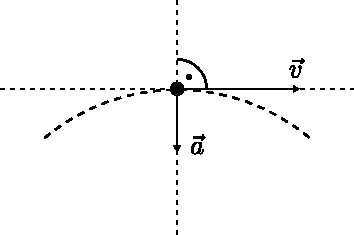
\includegraphics[scale=0.8]{bahnkurve.pdf}
	\caption{Bahnkurve mit Tangente und Normale dazu.}
	\label{fig:bahnkurve}
\end{figure}

\noindent
Betrachtet man die Grössen der Bewegung als Vektoren, so können diese 
in ihre jeweiligen Komponenten in $x,y,z$ zerlegt werden. Hierbei gilt 
insbesondere für die Geschwindigkeit $\vec{v}$ und die Beschleunigung
$\vec{a}$, dass diese entlang einer Bahnkurve stets normal zueinander 
sind oder anders formuliert:

\begin{itemize}
	\item Die Geschwindigkeit $\vec{v}$ liegt immer tangential an
		der Bahnkurve an.
	\item Gie Beschleunigung $\vec{a}$ zeigt immer nach innen, 
		d.h. normal zur Geschwindigkeit $\vec{v}$.
\end{itemize}

\section{Schiefer Wurf}
Der schiefe Wurf bezeichnet eine überlagerte Bewegung in mindestens zwei
Richtungen (z.B. $x$ und $y$). Diese Bewegung kann komponentenweise 
analysiert werden und per Superposition wieder zusammengesetzt werden.

\[\boxed{\begin{array}{r l  r l}
	& \vec{x}\text{-Komponente} & & \vec{y}\text{-Komponente} \\
	& & & \\
	\vec{a}_x 
		& = 0 
		& \qquad \vec{a}_y 
		& = -\vec{g} \\
	 & & &  \\
	\vec{v}_x 
		& = \vec{v}_0 \cdot cos(\alpha_0)
		& \vec{v}_y
		& = \vec{v}_0 \cdot sin(\alpha_0) -\vec{g} \cdot t \\
	 & & & \\
	\vec{s}_x
		& = \left( \vec{v}_0 \cdot cos(\alpha_0) \right) \cdot t
		& \vec{s}_y
		& = \left( \vec{v}_0 \cdot sin(\alpha_0) \right) \cdot t 
			- \frac{1}{2}\vec{g} \cdot t^2
\end{array}}\]

\noindent
Aus den obigen Zusammenhängen zum schiefen Wurf lässt sich eine 
Bahngleichung aufstellen, welche die Funktionen von $\vec{x}(t)$ und
$\vec{y}(t)$ kombiniert zu einer Funktion $\vec{y}(\vec{x})$.

\begin{figure}[h!]
	\centering
	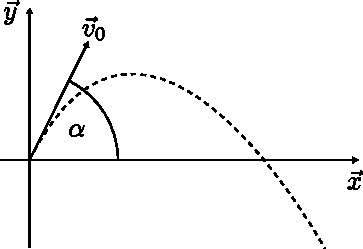
\includegraphics[scale=0.8]{wurf.pdf}
	\caption{Schiefer Wurf.}
	\label{fig:wurf}
\end{figure}

\[ \boxed{
	\vec{y} = \vec{x} \cdot tan(\alpha) 
		- \frac{\vec{g}}{2 \cdot \vec{v}_0^2 \cdot cos^2(\alpha)}
		\cdot \vec{x}^2
} \]

\noindent
Wichtig ist hierbei zu beachten, dass die passende Referenz für $\vec{y}$
gewählt wird, denn es gelten dann die folgenden Bedingungen.

\[ \boxed{\begin{array}{l l}
	\text{Landestelle tiefer als Abwurfstelle} & \Rightarrow y < 0 \\
	& \\
	\text{Landestelle gleich wie Abwurfstelle} & \Rightarrow y = 0 \\
	& \\
	\text{Landestelle höher als Abwurfstelle} & \Rightarrow y > 0 
\end{array}} \]


\subsection{Schräge Zerlegung}
Die Komponentenzerlegung eines Vektors kann beliebig erfolgen. 
D.h. die Zerlegung muss nicht zwingend in $x,y$ oder $z$ erfolgen,
sondern beliebig im Raum. Bei einigen Bewegungen ist dies von Vorteil,
etwa beim waagrechten Wurf (Spezialfall des schiefen Wurfs).

\begin{figure}[h!]
	\centering
	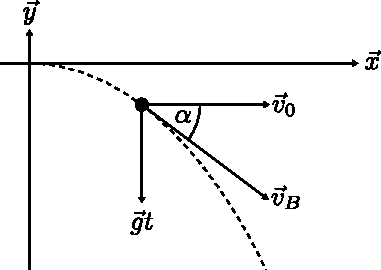
\includegraphics[scale=0.8]{wurf2.pdf}
	\caption{Schräge Komponentenzerlegung am waagrechten Wurf.}
	\label{fig:wurf2}
\end{figure}

\noindent
Mit dieser Zerlegung können die folgenden Zusammenhänge formuliert werden.
\[ \boxed{\begin{array}{r l}
	\vec{s} &
		= \vec{v}_0 \cdot t
		= \vec{v}_0 \cdot \sqrt{\frac{2 \cdot \vec{y}}{\vec{g}}} \\
	& \\
	\vec{y} &
		= \frac{1}{2} \cdot \vec{g} \cdot t^2 \\
	& \\
	\vec{v}_B &
		= \vec{v}_0 + \vec{g} \cdot t 
\end{array}}\]

    % Bewegung
% coding:utf-8

%----------------------------------------
%FOSAPHY, a LaTeX-Code for a summary of basic physics
%Copyright (C) 2013, Daniel Winz, Ervin Mazlagic

%This program is free software; you can redistribute it and/or
%modify it under the terms of the GNU General Public License
%as published by the Free Software Foundation; either version 2
%of the License, or (at your option) any later version.

%This program is distributed in the hope that it will be useful,
%but WITHOUT ANY WARRANTY; without even the implied warranty of
%MERCHANTABILITY or FITNESS FOR A PARTICULAR PURPOSE.  See the
%GNU General Public License for more details.
%----------------------------------------

\chapter{Rotation}
\section{Zentripetalkraft}
\[ F_z = \frac{m \cdot {v_b}^2}{r} = m \cdot \omega^2 \cdot r \]    % Rotation
% coding:utf-8

%----------------------------------------
%FOSAPHY, a LaTeX-Code for a summary of basic physics
%Copyright (C) 2013, Daniel Winz, Ervin Mazlagic

%This program is free software; you can redistribute it and/or
%modify it under the terms of the GNU General Public License
%as published by the Free Software Foundation; either version 2
%of the License, or (at your option) any later version.

%This program is distributed in the hope that it will be useful,
%but WITHOUT ANY WARRANTY; without even the implied warranty of
%MERCHANTABILITY or FITNESS FOR A PARTICULAR PURPOSE.  See the
%GNU General Public License for more details.
%----------------------------------------

\chapter{Reibung}

Die Reibung bezeichnet in der Pyhsik eine Eigenschaft, welche stets einer
Bewegung entgegenwirkt. In der Mechanik kann sie als Kraft verstanden
werden, welche zwischen sich berührenden Körpern auftritt. Hiebei gibt es
einige Arten der Reibung, die aufgrund ihres speziellen Charakters, 
unterschieden werden. Die wohl wichtigsten sind die Haft- und 
Gleitreibung (weiter gibt es z.B. noch die Roll-, Wälz-, Bohrreibung).

\newpage
\section{Reibungskraft}
Die Reibungskraft $\vec{F}_R$ ist eine Kraft welche zwischen sich
berührenden Körpern auftritt. Sie ist definiert als das Produkt aus
der Kraft $\vec{F}_N$ welche normal zwischen den Körpern anliegt
und dem Reibungskoeffizienten $\mu$ welcher die 
Oberflächenbeschaffenheit beschreibt. 

\begin{figure}[h!]
	\centering
	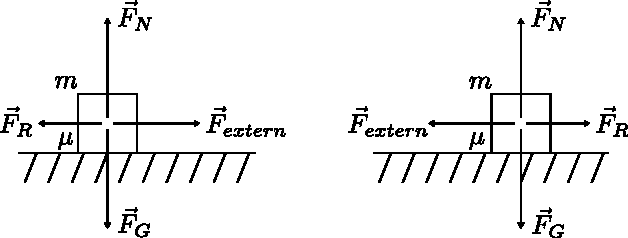
\includegraphics[scale=0.8]{reibung.pdf}
	\caption{Reibungskraft für eine Masse die auf einer Unterlage 
		liegt mit $\sum \vec{F}_{extern}$ positiv (l)
		und negativ (r).}
\end{figure}

\noindent
Die Richtung der Reibungskraft ist dabei stets entgegen der 
anliegenden äusseren Nettokraft 
$\sum \vec{F}_{extern}$.

\[ \boxed{
	\vec{F}_R = \vec{F}_N \cdot \mu
		\qquad ,\vec{F}_R \bot \vec{F}_N
}\]

\section{Bewegungsbedingung}
\noindent
Ein Körper der eine Reibung kennt, bringt eine Kraft $\vec{F}_R$ 
auf entgegen der anliegenden Nettokraft $\sum \vec{F}_{extern}$. 
Das bedeutet, dass ein solcher Körper in Ruhe bleibt, solange die 
anliegende Nettokraft $\sum \vec{F}_{extern} \leq \vec{F}_R$ ist. 
Somit ergibt sich die Bewegungsbedingung zu

\[ \boxed{\begin{array}{l r l}
	\text{Körper bleibt in Ruhe falls } & 
		\sum \vec{F}_{extern} & \leq \vec{F}_R \\
	& & \\
	\text{Körper bewegt sich falls } &
		\sum \vec{F}_{extern} & > \vec{F}_R 
\end{array}} \]

\section{Reibungskoeffizient}
Der Reibungskoeffizient $\mu$ wird typischerweise für zwei Fälle 
angegeben, welche voneinander zu unterscheiden sind.
\begin{itemize}
	\item Haften $\Rightarrow$ Haftreibungskoeffizient $\mu_{HR}$
	\item Gleiten $\Rightarrow$ Gleitreibungskoeffizient $\mu_{GR}$
\end{itemize}

\noindent
Für den Reibungskoeffizienten gilt stets, dass der Koeffizient für die
Haftung grösser oder zumindest gleich ist wie für das Gleiten 
(bei den selben Bedingungen).

\[ \boxed{
	\mu_{HR} \geq \mu_{GR}
}\]

\begin{footnotesize}
\begin{longtable}{llll}
  \rowcolor{white} \textbf{Material 1} & \textbf{Material 2} 
  & \textbf{Haftreibung $\mu_{HR}$} & \textbf{Gleitreibung $\mu_{GR}$}\\
  \rowcolor{lgray}  Stahl     & Stahl             & 0.74 & 0.57\\
  \rowcolor{white}  Aluminium & Stahl             & 0.61 & 0.47\\
  \rowcolor{lgray}  Kupfer    & Stahl             & 0.53 & 0.36\\
  \rowcolor{white}  Messing   & Stahl             & 0.51 & 0.44\\
  \rowcolor{lgray}  Zink      & Grauguss          & 0.85 & 0.21\\
  \rowcolor{white}  Kupfer    & Grauguss          & 1.05 & 0.29\\
  \rowcolor{lgray}  Glas      & Glas              & 0.94 & 0.40\\
  \rowcolor{white}  Kupfer    & Glas              & 0.68 & 0.53\\
  \rowcolor{lgray}  Teflon    & Teflon            & 0.04 & 0.04\\
  \rowcolor{white}  Teflon    & Stahl             & 0.04 & 0.04\\
  \rowcolor{lgray}  Gummi     & Beton (trocken)   & 1.0  & 0.80\\
  \rowcolor{white}  Gummi     & Beton (nass)      & 0.30 & 0.25
\end{longtable}
\end{footnotesize}

     % Reibung
% coding:utf-8

%----------------------------------------
%FOSAPHY, a LaTeX-Code for a summary of basic physics
%Copyright (C) 2013, Daniel Winz, Ervin Mazlagic

%This program is free software; you can redistribute it and/or
%modify it under the terms of the GNU General Public License
%as published by the Free Software Foundation; either version 2
%of the License, or (at your option) any later version.

%This program is distributed in the hope that it will be useful,
%but WITHOUT ANY WARRANTY; without even the implied warranty of
%MERCHANTABILITY or FITNESS FOR A PARTICULAR PURPOSE.  See the
%GNU General Public License for more details.
%----------------------------------------

\chapter{Schwingung}
\section{Begriffe}
\begin{tabular}{ll}
$\omega:$       & Kreisfrequenz \\
$f:$            & Frequenz \\
$T:$            & Periodendauer \\
$A:$            & Amplitude \\
$\phi:$         & Phasenverschiebung \\
$x:$            & Auslenkung \\
$\theta:$       & Auslenkwinkel \\
$I:$            & Trägheitsmoment $[kg m^2]$ \\
$k:$            & Federkonstante $[\frac{N}{m}]$ \\
$\kappa:$       & Rotationsfederkonstante $[Nm]$ \\
$d:$            & Abstand Massenschwerpunkt zu Drehachse \\
$L:$            & Pendellänge \\
$\ell:$         & Länge der Flüssigkeitssäule \\
$\beta:$        & Abklingkonstante $[s^{-1}]$ \\
$b:$            & Dämpfungskonstante $[\frac{kg}{s}]$ \\
$\tau:$         & Zeitkonstante, Zerfallszeit $[s]$ \\
$Q:$            & Güte \\
$H:$            & Erregerauslenkung \\
$\Omega_R:$     & Resonanzkreisfrequenz \\
$\Delta\Omega:$ & Kurvenbreite, Bandbreite \\
\end{tabular}

%\section{Einfache harmonische Schwingung}
% coding:utf-8

%----------------------------------------
%FOSAPHY, a LaTeX-Code for a summary of basic physics
%Copyright (C) 2013, Daniel Winz, Ervin Mazlagic

%This program is free software; you can redistribute it and/or
%modify it under the terms of the GNU General Public License
%as published by the Free Software Foundation; either version 2
%of the License, or (at your option) any later version.

%This program is distributed in the hope that it will be useful,
%but WITHOUT ANY WARRANTY; without even the implied warranty of
%MERCHANTABILITY or FITNESS FOR A PARTICULAR PURPOSE.  See the
%GNU General Public License for more details.
%----------------------------------------

\section{Einfache harmonische Schwingung}
Die einfache harmonische Schwingung beschreibt ein System, welches 
nur zwei Energiespeicher hat. Ein klassisches Beispiel
ist die an einer Feder befestigte Masse. Um ein 
schwingfähiges System zu erhalten, muss es Wirkungen geben welche
entgegengesetzt sind. Im Beispiel aus Abbildung 
\ref{fig:einfache-harmonische} gibt es die zwei Kräfte $\vec{F}_k$ und
$\vec{F}_m$ die entgegengesetzt sind.

\begin{figure}[h!]
	\centering
	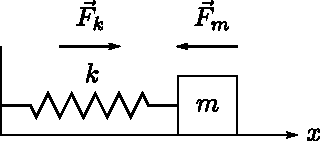
\includegraphics[scale=0.75]{../fig/einfache-harmonische.pdf}
	\caption{Einfach harmonisches Schwinungssystem}
	\label{fig:einfache-harmonische}
\end{figure}

\begin{figure}[h!]
	\centering
	\begin{tikzpicture}[domain=0:4]
		\draw[->] (-0.1,0) -- (5,0) node[below] {$t$};
		\draw[->] (0,-2.5) -- (0,2.5) node[left] {$x$};

		\draw[color=red, samples=200] plot[id=x] 
			function{0.5*cos(2*x)};
		\draw[color=blue, samples=200] plot[id=v] 
			function{-2*0.5*sin(2*x)};
		\draw[color=green, samples=200] plot[id=a] 
			function{-2*2*0.5*cos(2*x)};

		\draw[red] (4,2) node[right] 
			{$x(t) = A \sin(\omega t + \varphi)$};
		\draw[blue] (4,1.5) node[right] 
			{$\dot{x}(t) = -\omega A \cos(\omega t + \varphi)$};
		\draw[green] (4,1) node[right]
			{$\ddot{x}(t) = -\omega^2 A \sin(\omega t + \varphi)$};

		\draw[] (0.1,0.5) -- (-0.1,0.5) node[left] {$A$};
		\draw[] (0.1,1) -- (-0.1,1) node[left] {$\omega A$};
		\draw[]	(0.1,2) -- (-0.1,2) node[left] {$\omega^2 A$};
	\end{tikzpicture}
	\caption{Plot der einfachen harmonischen Schwingung}
\end{figure}

\subsection{Differentialgleichung}
Der Zusammenhang aus Abbildung \ref{fig:einfache-harmonische} stellt 
direkt die allgemeine Form des Systems als Differentialgleichung auf zu
\[ \boxed{\vec{F}_\Sigma  
	= \vec{F}_m + \vec{F}_k
	= m \cdot \ddot{x} + k \cdot x
	= 0
} \]

Der Weg, die Geschwindigkeit und die Beschleunigung lassen sich analog
zur linearen Bewegung durch Ableitungen und Integrale voneinander herleiten.
\[ \boxed{ \begin{array}{c c l}
	x(t) & = & 
		A \cdot \cos(\omega \cdot t + \varphi) \\
	\dot{x}(t) & = & 
		-\omega A \cdot \sin(\omega \cdot t + \varphi) \\
	\ddot{x}(t) & = & 
		-\omega^2 A \cdot \cos(\omega \cdot t + \varphi)
\end{array}}\]

Die Amplitude $A$ und die Phasenverschiebung $\varphi$ bietet die  
Parametierung der Bewegung an. Diese sind bei der einfachen harmonischen 
und ungedämpften Schwingung stets konstant. Die Kreisfrequenz $\omega$ 
beschreibt die Dynamik des Systems, also die \textit{Schnelligkeit}.
Diese kann aber auch mittels der Frequenz $f$ oder der Periodendauer $T$
ausgedrückt werden. 
\[ \boxed{ 
	\omega = 2 \pi f = 2 \pi \frac{1}{T}
	\quad \Rightarrow \quad
	f = \frac{\omega}{2 \pi} 
	\quad \Rightarrow \quad 
	T = \frac{2 \pi}{\omega} = \frac{1}{f} \\
} \]
Bei einfachen harmonischen Systemen wie in Abbildung 
\ref{fig:einfache-harmonische} ist die Dynamik definiert durch das
Verhältnis von Feder und Masse.
\[ \boxed{
	\omega = \sqrt{\frac{k}{m}}
}\]

\subsection{Auslenkung und Geschwindigkeit als Anfangsbedingungen}
Wird die Feder vor dem loslassen um die Strecke $x_0$ gedehnt, gibt 
dies die Amplitude $A$ vor. 
\[ \boxed{A = \sqrt{{x_0}^2 + \left(\frac{v_0}{\omega}\right)^2}} \]
\[ \boxed{x_0 = x(0) = A \cdot \cos(\varphi)} \]
Wird die Masse nicht einfach losgelassen
sondern mit einer Geschwindigkeit $\vec{v}_0$ bewegt, dann gibt dies
die Phasenverschiebung $\varphi$ vor.
\[ \boxed{v_0 = \dot{x}(0) = - \omega \cdot A \cdot \sin(\varphi)} \]
\[ \boxed{\phi = \tan^{-1}\left(-\frac{v_0}{\omega \cdot x_0}\right)} \]
\textbf{Achtung!} Lösung kann im falschen Quadranten liegen. 
Evtl. mit $\pi$ addieren. 


\subsection{Geschwindigkeit und Beschleunigung aus Amplitude und Position}
\[ \boxed{v(t) = \sqrt{\frac{k}{m}} \cdot \sqrt{A^2 - x^2(t)}
	= \omega \sqrt{A^2 - x^2(t)}} \]
\[ \boxed{a(t) = - \frac{k}{m} \cdot x(t) = - \omega^2 x(t)} \]

\subsection{Maximale Geschwindigkeit und Beschleunigung}
\[ \boxed{v_{max} = \omega \cdot A} \]
\[ \boxed{v_{min} = -\omega \cdot A} \]
\[ \boxed{a_{max} = -\omega^2 \cdot A} \]

\subsection{Vertikales Federpendel}
Das vertikale Federpendel beschreibt das selbe harmonische System wie in
Abbildung \ref{fig:einfache-harmonische}. Der Unterschied liegt allein 
darin, dass die Gleichgewichtslage verschoben ist, da die Erdbeschleunigung 
wirkt und die Feder gedehnt wird.

\begin{figure}[h!]
	\centering
	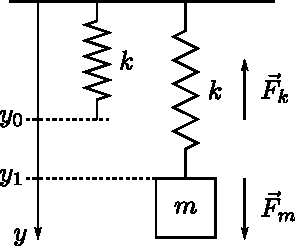
\includegraphics[scale=0.75]{../fig/federpendel-vertikal.pdf}
	\caption{Vertikales Federpendel}
	\label{fig:federpendel-vertikal}
\end{figure}

Der Einfluss der Erdbeschleunigung zeigt sich als \textit{Offset} in
der Bewegungsgleichung
\[ \boxed{x(t) = \underbrace{-\frac{m \cdot g}{k}}_{\text{Offset}} 
	+ A \cdot \cos(\omega \cdot t + \phi)} \]
Die Dynamik des Systems ist jedoch nicht beeinflusst von diesem 
Offset, da die Bewegung die selbe bleibt.
\[ \boxed{\omega = \sqrt{\frac{k}{m}}} \]

\subsection{Energie}
Die Energie eines einfach harmonischen Schwingungssystems verlagert
sich ständig zwischen den beiden Energiespeichern. In den Extremlagen,
also dort wo die Geschwindigkeit maximal und minimal ist, ist die
gesamte Energie jeweils in der Feder bzw. in der Bewegung (kinetische
Energie).
\[ \boxed{E_{pot}(t) = \frac{1}{2} \cdot k \cdot x(t)^2} \]
\[ \boxed{E_{kin}(t) = \frac{1}{2} \cdot m \cdot v(t)^2} \]
Möchte man die Gesamtenergie des Systems so kann man dies für eine
der Extremlagen mittels einer der obigen Formeln berechnen. Für eine
beliebige Lage muss hierfür eine Kombination aus beiden Energien
berechnet werden.
\[ \boxed{E_{tot} = \frac{1}{2} \cdot k \cdot A^2 
= \frac{1}{2} \cdot m \cdot \omega^2 \cdot A^2 
= \frac{1}{2} \cdot m \cdot (v_{max})^2} \]



\begin{comment}
Differentialgleichung: 
\[ \boxed{F = m \cdot \ddot{x} + k \cdot x = 0} \]
\[ \boxed{x(t) = A \cdot \cos(\omega \cdot t + \phi)} \]
\[ \boxed{\dot{x}(t) = - \omega A \cdot \sin(\omega \cdot t + \phi)} \]
\[ \boxed{\ddot{x}(t) = - \omega^2 A \cdot \cos(\omega \cdot t + \phi)} \]
\[ \boxed{\omega = \sqrt{\frac{k}{m}} = 2 \pi f} \]
\[ \boxed{f = \frac{\sqrt{\dfrac{k}{m}}}{2 \pi} = \frac{\omega}{2 \pi} } \]
\[ \boxed{T = 2 \cdot \pi \sqrt{\frac{m}{k}} = \frac{1}{f} } \]

\subsection{Auslenkung und Geschwindigkeit als Anfangsbedingungen}
\[ \boxed{x_0 = x(0) = A \cdot \cos(\phi)} \]
\[ \boxed{v_0 = \dot{x}(0) = - \omega \cdot A \cdot \sin(\phi)} \]
\[ \boxed{\phi = \tan^{-1}\left(-\frac{v_0}{\omega \cdot x_0}\right)} \]
\textbf{Achtung!} Lösung kann im falschen Quadranten liegen. 
Evtl. mit $\pi$ addieren. 
\[ \boxed{A = \sqrt{{x_0}^2 + \left(\frac{v_0}{\omega}\right)^2}} \]

\subsection{Geschwindigkeit und Beschleunigung aus Amplitude und Position}
\[ \boxed{v(t) = \sqrt{\frac{k}{m}} \cdot \sqrt{A^2 - x^2(t)}
	= \omega \sqrt{A^2 - x^2(t)}} \]
\[ \boxed{a(t) = - \frac{k}{m} \cdot x(t) - \omega^2 x(t)} \]

\subsection{Maximale Geschwindigkeit und Beschleunigung}
\[ \boxed{v_{max} = \omega \cdot A} \]
\[ \boxed{v_{min} = -\omega \cdot A} \]
\[ \boxed{a_{max} = -\omega^2 \cdot A} \]

\subsection{Vertikales Federpendel}
\[ \boxed{\omega = \sqrt{\frac{k}{m}}} \]
\[ \boxed{x(t) = - \frac{m \cdot g}{k} + A \cdot \cos(\omega \cdot t + \phi)} \]

\subsection{Energie}
\[ \boxed{E_{pot}(t) = \frac{1}{2} \cdot k \cdot x(t)^2} \]
\[ \boxed{E_{kin}(t) = \frac{1}{2} \cdot m \cdot v(t)^2} \]
\[ \boxed{E_{tot} = \frac{1}{2} \cdot k \cdot A^2 
= \frac{1}{2} \cdot m \cdot \omega^2 \cdot A^2 
= \frac{1}{2} \cdot m \cdot (v_{max})^2} \]
\end{comment}


%\section{Rotationsschwingung}
\section{Rotationsschwingung}
Die Rotationsschwingung ist wie das horizontale und vertikale Federpendel
ein einfach harmonisches Schwingungssystem. Dies zeigt sich direkt an deren
Differentialgleichung. Da es sich hier um eine Rotationsbewegung handelt 
wird diese mittels der Momente gebildet
\[ \boxed{\vec{M}_{\Sigma} 
	= \vec{M}_R + \vec{M}_F 
	= I_s \cdot \ddot{\theta} + \kappa \cdot \theta = 0
} \]
\[ \boxed{\theta(t) = \theta_{max} \cdot \cos(\omega \cdot t + \phi)} \]

\begin{figure}[h!]
	\centering
	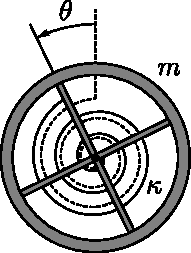
\includegraphics[scale=0.75]{../fig/rotationspendel.pdf}
	\caption{Rotationspendel}
\end{figure}

\paragraph{Spiralfeder} Im Unterschied zur Linearfeder wird die Spiralfeder
nicht mittels eines $k=\left[\frac{N}{m}\right]$ sondern mittels eines
$\kappa=\left[Nm\right]$ beschrieben.

\paragraph{Für kleine Winkel} Ist die Auslenkung $\theta$ klein, dann gelten
 die folgenden Formeln.
\[ \boxed{\kappa = \sum_{1}^{n} \left(k_n \cdot {r_n}^2\right)} \]
\[ \boxed{\kappa = k_1 \cdot {r_1}^2 + k_2 \cdot {r_2}^2 + \dots } \qquad 
\text{$r$: Abstand Feder zu Drehpunkt} \]
\[ \boxed{\omega = \sqrt{\frac{\kappa}{I}}} \]
\[ \boxed{f = \frac{\sqrt{\dfrac{\kappa}{I}}}{2 \pi}} \]
\[ \boxed{T = 2 \cdot \pi \cdot \sqrt{\frac{I}{\kappa}}} \]

\begin{comment}
Differentialgleichung: 
\[ \boxed{M = I_s \cdot \ddot{\theta} + \kappa \cdot \theta = 0} \]
\[ \boxed{\theta(t) = \theta_{max} \cdot \cos(\omega \cdot t + \phi)} \]
für kleine Winkel: 
\[ \boxed{\kappa = k_1 \cdot {r_1}^2 + k_2 \cdot {r_2}^2 + \dots } \qquad 
\text{$r$: Abstand Feder zu Drehpunkt} \]
\[ \boxed{\kappa = \sum_{1}^{n} \left(k_n \cdot {r_n}^2\right)} \]
\[ \boxed{\omega = \sqrt{\frac{\kappa}{I}}} \]
\[ \boxed{f = \frac{\sqrt{\dfrac{\kappa}{I}}}{2 \pi}} \]
\[ \boxed{T = 2 \cdot \pi \cdot \sqrt{\frac{I}{\kappa}}} \]
\end{comment}

%\section{Physikalisches Pendel}
\section{Physikalisches Pendel}
Das physikalische Pendel ist wie das Rotationspendel ein einfach harmonisches 
Schwingungssystem. Wie zuvor wird hier die Differentialgelichung mittels der
Momente aufgestellt. 
\[ \boxed{\vec{M}_{\Sigma} 
	= \vec{M}_k + \vec{M}_g	
	= I_z \cdot \ddot{\theta} + d \cdot m \cdot g \cdot \sin(\theta) = 0
} \]
Für kleine Winkel $\theta$ kann $\sin(\theta)$ mit $\theta$ approxmiert
werden.
\[ \boxed{ \sin(\theta) \approx \theta \quad\text{falls }\theta\text{ klein}
} \]
Mit dieser Approximation lässt sich die Differentialgleichung vereinfachen 
zu 
\[ \boxed{M 
	= I_z \cdot \ddot{\theta} + d \cdot m \cdot g \cdot \theta 
	= 0
} \]

\begin{figure}[h!]
	\centering
	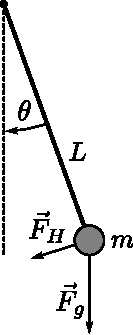
\includegraphics[scale=0.75]{../fig/physikalisches-pendel.pdf}
	\caption{Physikalisches Pendel}
	\label{fig:physikalisches-pendel}
\end{figure}

Das Verhalten ist analog zu den anderen einfach harmonischen 
Schwingungssystemen.
\[ \boxed{\kappa = d \cdot m \cdot g} \qquad 
\text{Schwerpunkt über Drehachse $\Rightarrow$ $\kappa$ negativ} \]
\[ \boxed{\kappa_{tot} = \kappa_1 + \kappa_2 \dots} \]
\[ \boxed{\kappa_{tot} = \sum_{1}^{n} \left(d_n \cdot m_n \cdot g\right) } \]
\[ \boxed{\omega = \sqrt{\frac{\kappa}{I_z}} 
= \sqrt{\frac{m \cdot g \cdot d}{I_z}}} \]
\[ \boxed{f = \frac{\sqrt{\frac{\kappa}{I_z}}}{2 \pi}
= \frac{\sqrt{\frac{m \cdot g \cdot d}{I_z}}}{2 \pi}} \]
\[ \boxed{T = 2 \cdot \pi \cdot \sqrt{\frac{I_z}{m \cdot g \cdot d}}} \]

\subsection{Fadenpendel}
Ein Spezialfall des pysikalischen Pendels ist das sog. Fadenpendel. 
Dies ist ein Pendel, welches einen Massepunkt am Ende eines masselosen
Seils hat. Das Trägheitsmoment bildet sich somit aus einem rein 
steiner'schen Anteil (siehe \textit{Satz von Steiner}, 
Seite \pageref{sec:steiner}).
\[ \boxed{I = m \cdot L^2} \]
Das Verhalten des Systems ist analog zum allgemeinen physikalischen
Pendel. Die Formel sind lediglich vereinfacht durch das spezielle
Trägheitsmoment.
\[ \boxed{\kappa = m \cdot g \cdot L} \]
\[ \boxed{\omega = \sqrt{\frac{g}{L}}} \]
\[ \boxed{f = \frac{\sqrt{\frac{g}{L}}}{2 \cdot \pi}} \]
\[ \boxed{T = 2 \cdot \pi \cdot \sqrt{\frac{L}{g}}} \]
Die Kraft im Seil setzt sich zusammen aus den Radialanteilen der
wirkenden Kräfte.
\[ \boxed{\vec{F}_s 
	= \underbrace{ 
		m \cdot g \cdot \cos(\theta)
	}_{\substack{\text{Radialanteil}\\\text{Gewichtskraft}}}
	+ \underbrace{
		m \cdot \frac{v^2}{L}
	}_{\substack{\text{Radialanteil}\\\text{Rotation}}}
	= m \cdot g \cdot \cos(\theta) + m \cdot \omega^2 \cdot L
} \]


\begin{comment}
Differentialgleichung: 
\[ \boxed{M = I_z \cdot \ddot{\theta} + d \cdot m \cdot g \cdot \sin(\theta) = 0} \]
für kleine Winkel $\theta$ gilt $\sin(\theta) \approx \theta$: 
\[ \boxed{M = I_z \cdot \ddot{\theta} + d \cdot m \cdot g \cdot \theta = 0} \]
\[ \boxed{\kappa = d \cdot m \cdot g} \qquad 
\text{Ist der Schwerpunkt über dem Drehpunkt, ist $\kappa$ negativ} \]
\[ \boxed{\kappa_{tot} = \kappa_1 + \kappa_2 \dots} \]
\[ \boxed{\kappa_{tot} = \sum_{1}^{n} \left(d_n \cdot m_n \cdot g\right) } \]
\[ \boxed{\omega = \sqrt{\frac{\kappa}{I_z}} 
= \sqrt{\frac{m \cdot g \cdot d}{I_z}}} \]
\[ \boxed{f = \frac{\sqrt{\frac{\kappa}{I_z}}}{2 \pi}
= \frac{\sqrt{\frac{m \cdot g \cdot d}{I_z}}}{2 \pi}} \]
\[ \boxed{T = 2 \cdot \pi \cdot \sqrt{\frac{I_z}{m \cdot g \cdot d}}} \]
speziell: Fadenpendel
\[ \boxed{I = m \cdot L^2} \]
\[ \boxed{\kappa = m \cdot g \cdot L} \]
\[ \boxed{\omega = \sqrt{\frac{g}{L}}} \]
\[ \boxed{f = \frac{\sqrt{\frac{g}{L}}}{2 \cdot \pi}} \]
\[ \boxed{T = 2 \cdot \pi \cdot \sqrt{\frac{L}{g}}} \]
Fadenkraft: 
\[ \boxed{F_s = m \cdot g \cdot \cos(\theta) + m \cdot \frac{v^2}{L} 
= m \cdot g \cdot \cos(\theta) + m \cdot \omega^2 \cdot L} \]
\end{comment}

\section{Pendelnde Flüssigkeitssäule}
\[ \boxed{\omega = \sqrt{\frac{2 \cdot g}{\ell}}} \]
\[ \boxed{f = \frac{\sqrt{\frac{2 \cdot g}{\ell}}}{2 \pi}} \]
\[ \boxed{T = 2 \pi \sqrt{\frac{\ell}{2 \cdot g}}} \]

\section{Gedämpfte Schwingung}
Differentialgleichung: 
\[ \boxed{F = m \cdot \ddot{x} + \underbrace{b \cdot \dot{x}}_
{\text{Dämpfung}} + k \cdot x = 0} \]
\[ \boxed{F_{\text{Dämpfung}} = F_{\text{Stokes}} 
= 6 \pi \cdot \eta \cdot R \cdot v} \]
\[ \boxed{\rightarrow b = 6 \pi \cdot \eta \cdot R} \]
\[ \boxed{\omega = \sqrt{\frac{k}{m}}} \]
\[ \boxed{\beta = \frac{b}{2 m}} \]
Fall 1: $\beta > \omega$ "'Kriechfall"'
\[ \boxed{x(t) \sim e^{(-\beta \pm \delta)t}} \]
Fall 2: $\beta = \omega$ "'kritische Dämpfung"'
\[ \boxed{b = b_{krit} = \sqrt{4 \cdot k \cdot m}} \]
Fall 3: $\beta < \omega$ "'Gedämpfte Schwingung"'
\[ \boxed{x(t) = A \cdot e^{-\beta t} \cdot \cos(\omega_d \cdot t)} \]
\[ \boxed{\omega_d = \sqrt{\omega^2 - \beta^2} 
= \sqrt{\frac{k}{m} - \left({\frac{b}{2 \cdot m}}\right)^2}} \]
Zerfallszeit: 
\[ \boxed{\tau = \frac{1}{\beta}} \]
\[ \boxed{A(t) = A_0 \cdot e^{-\beta t} = A_0 \cdot e^{-\frac{t}{\tau}}} \]
Bei der Zeit $t = \tau$
\[ \boxed{A(\tau) = \frac{A_0}{e} = A_0 \cdot e^{-1} \approx 0.37 \cdot A_0} \]
Abklingkonstante: 
\[ \boxed{\beta 
= \frac{\ln\left(\frac{x(t_1)}{x(t_2)}\right)}{t_2 - t_1}} \]
Schwingungsenergie: 
\[ \boxed{E(t) = \frac{m}{2} \cdot \dot{x}^2(t) + \frac{k}{2} \cdot x^2(t)} \]
Mittlere Energie: 
\[ \boxed{\langle E(t)\rangle = E_0 \cdot e^{-\frac{2 \cdot t}{\tau}}} \]
Güte: 
\[ \begin{array}{l}
\boxed{Q = \frac{2 \pi \cdot E(t)}{|\Delta E(t)|} 
= \frac{\pi}{\beta \cdot T_d} = \frac{\pi \cdot \tau}{T_d} 
= \frac{\omega_d \cdot \tau}{2}} \\
\text{$\Delta E(t)$: Energieverlust pro Periode}
\end{array} \]

\section{Erzwungene Schwingung}
\[ \boxed{x(t) = A(\Omega) \cdot \cos(\Omega t - \varphi(\Omega))} \]
\[ \boxed{A(\Omega) = \frac{F_0}{m \cdot 
\sqrt{(\omega^2 - \Omega^2)^2 + (2 \cdot \Omega \cdot \beta)^2}} 
\approx \frac{H}{\sqrt{\left(1 - \left(\frac{\Omega}{\omega}\right)^2\right)^2 
+ \left(\frac{\Omega}{Q \cdot \omega}\right)^2}}} \]  
\[ F_0\text{: Anregungskraft} \qquad H\text{: Anregungsamplitude} \]
\[ \boxed{\varphi(\Omega) = \arctan\left(\frac{2 \cdot \Omega \cdot \beta}
{{\omega}^2 - \Omega^2}\right) 
= \arctan{\left(\frac{\frac{b}{\sqrt{k \cdot m}} 
\left(\frac{\Omega}{\omega}\right)}
{1 - \left(\frac{\Omega}{\omega}\right)^2}\right)}} \]
\[ \boxed{H = \frac{F_0}{k}} \]
\[ \boxed{\omega = \sqrt{\frac{k}{m}}} \]
\[ \boxed{\beta = \frac{b}{2 m} = \frac{1}{\tau}} \]
\[ \boxed{Q = \frac{\omega_d}{2\beta} = \omega_d \frac{m}{b} 
= \pi \frac{\tau}{T}} \]
schwache Dämpfung: 
\[ \boxed{b << b_{krit} = \sqrt{4 k \cdot m} \quad Q >> 1} \]

\subsection{Resonanzfrequenz}
\[ \boxed{\Omega_R = \sqrt{\omega^2 - 2\beta^2} \neq \omega_d 
= \sqrt{\omega^2 - \beta^2} \neq \omega} \]
\[ \boxed{A(\Omega_R) = \frac{\omega^2 H}{2 \beta \sqrt{\omega^2 - \beta^2}} 
= \frac{k H}{m \sqrt{(\omega^2 - {\Omega_R}^2)^2 + (2\beta\Omega_R)^2}} 
\approx \frac{Q H}{\sqrt{1 - \frac{1}{2 Q^2}}} \approx Q \cdot H} \]
\[ \boxed{\varphi_R = \varphi(\Omega_R) 
= \arctan\left(\frac{2 \beta \omega_R}{\omega^2 - {\Omega_R}^2}\right) 
\approx \arctan\left(\sqrt{4 Q^2 - 2}\right) \approx \frac{\pi}{2}} \]
Für $Q>5$
\[ \boxed{\Omega_R \approx \omega \left(1 - \frac{1}{4Q^2}\right)} \]
\[ \boxed{A_R = A(\Omega_R) \approx \frac{Q H}{\sqrt{1 - \frac{1}{2Q^2}}} 
\approx Q \cdot H} \]
\[ \boxed{Q \approx \frac{\Omega_R}{\Delta\Omega}} \]
  % Schwingung
% coding:utf-8

%----------------------------------------
%FOSAPHY, a LaTeX-Code for a summary of basic physics
%Copyright (C) 2013, Daniel Winz, Ervin Mazlagic

%This program is free software; you can redistribute it and/or
%modify it under the terms of the GNU General Public License
%as published by the Free Software Foundation; either version 2
%of the License, or (at your option) any later version.

%This program is distributed in the hope that it will be useful,
%but WITHOUT ANY WARRANTY; without even the implied warranty of
%MERCHANTABILITY or FITNESS FOR A PARTICULAR PURPOSE.  See the
%GNU General Public License for more details.
%----------------------------------------

\chapter{Wellen}
\section{Allgemein}
\[ \boxed{f(x,t) = f^*(x \pm v \cdot t} \]
      % Wellen

\end{document}

